% Overview:
%   DiscoSNP++ TeX subfile for the project.
%   Each subfile MUST start with the following line
%		\documentclass[../main.tex]{subfiles}

\documentclass[../main.tex]{subfiles}

\begin{document}

\subsection{DiscoSnp\texttt{++}}
\label{discosnp++}

Il secondo framework che viene presentato è DiscoSnp\texttt{++} \cite{peterlongo2017discosnp++}; rientra nella categoria dei metodi \textit{hybrid}, ed è stato presentato come la nuova versione di \textsc{DiscoSnp} \cite{uricaru2015reference}, framework che si proponeva di individuare SNP isolati eterozigoti e omozigoti. DiscoSnp\texttt{++} è stato reimplementato da zero usando la libreria GATB \cite{drezen2014gatb} e permette di ottenere un tempo di esecuzione più veloce ed un minor consumo di memoria rispetto alla sua precedente versione. È stato progettato per individuare e classificare, senza utilizzare un genoma di riferimento, tutte le tipologie di SNP, compresi piccoli indel provenienti direttamente dalle read sequenziate (formato FastQ\footnote{\ Nota \vref{nota:FASTQ}} o FASTA) differentemente da \textsc{DiscoSnp} che era specializzato nella classificazione di una sola tipologia di SNP.

Normalmente DiscoSnp\texttt{++} restituisce gli SNP individuati e classificati nel formato VCF, ma opzionalmente può restituirli dopo averli mappati su un genoma di riferimento. Questo può inizialmente apparire in contrasto con un approccio \textit{reference free}, tuttavia torna particolarmente utile quando si dispone di un genoma di riferimento che non può essere usato per effettuare la chiamata delle varianti tramite tecniche di mappatura ma che può essere usato per posizionare le varianti predette tramite tecniche \textit{de-novo}. In situazioni abbastanza comuni, queste casistiche si presentano quando il genoma di riferimento è stato assemblato male o si sta analizzando un genoma molto distante dalla specie sequenziata. In ogni caso, anche se ci fosse un buon genoma di riferimento, la predizione delle varianti e la genotipizzazione con l'approccio reference free non sono influenzate in alcun modo dagli alleli di riferimento.

\subsubsection{Una struttura dati per identificare varianti: il grafo di \textit{de Bruijn}}
\label{dBG}

I grafi di \textit{de Bruijn} sono la struttura dati su cui si basano la maggior parte dei tool \textit{reference free} per la  ricerca di mutazioni (SNP) senza l'utilizzo dell'allinemento, in quanto eliminano la necessità di un genoma di riferimento e utilizzando direttamente i confronti della sequenza grezza.

\theoremstyle{definition}
\begin{definition} 
Dato un insieme di stringhe $S = \{r_1 , r_2 , ... , r_n\}$ su un alfabeto $\Sigma$ ed un intero $k\geq2$, il grafo di \textit{de Bruijn} di ordine $k$ di $S$ $(dBG_k (S))$ è un grafo diretto (o digrafo) $(V,A)$ dove:
\begin{itemize}
\item[-] $V = \{d \in \Sigma^k \ |\  \exists i \in \{1, ..., n\} \ tale\ che\ d\ \grave{e}\ una\ sottostringa\ di\ r_i \in S\}$
\item[-]$A = \{ (d,d^\prime)\ |\ se\ il\ suffisso\ di\ lunghezza\ k-1\ di\ d\ \grave{e}\ prefisso\ di\ d^\prime\}$
\end{itemize}
\end{definition}

\noindent
I grafi di \textit{de Bruijn} sono quindi grafi diretti che ben si adattano a rappresentare relazioni ordinate tra sequenze della stessa lunghezza, come \textit{k}-mer delle read (vedi Figura \ref{fig:dBG}) ed hanno inoltre dimostrato di essere di grande utilità come modello di dati; su di esso sono stati implementati quasi tutti gli algoritmi di assemblaggio \textit{de novo} progettati per utilizzare dati provenienti da \textit{short read}. Alcuni esempi degni di nota di questi algoritmi sono Velvet e ABySS. Nella maggior parte di questi strumenti di assemblaggio, il grafo di \textit{de Bruijn} è implementato come una struttura dati interna che rappresenta una rete in cui i nodi contengono i \textit{k}-mer delle read e i gli archi contengono i ($k-1$) nucleotidi sovrapposti tra i \textit{k}-mer\footnote{\ Dipendentemente dalla definizione con cui si costruisce il grafo di \textit{de Bruijn}, il \textit{k}-mer può essere il nodo o l'arco che congiunge due nodi. \textbf{Definizione nodo-centrica}: i nodi sono tutte le sottostringhe di lunghezza \textit{k} di ogni stringa in $S$. Un arco $s_1 \rightarrow s_2$ è presente se il suffisso di lunghezza ($k-1$) di $s_1$ è anche un prefisso di $s_2$. \textbf{Definizione arco-centrica}: tra i $k^\prime$-mer (nodi), un arco $s_1 \rightarrow s_2$ è presente se esiste un $(k^\prime+1)$-mer in una stringa di $S$ che contiene $s_1$ come prefisso e $s_2$ come suffisso. Le definizioni nodo-centriche e arco-centriche sono essenzialmente equivalenti quando $k^\prime = k-1$ (anche se nella prima i nodi hanno lunghezza \textit{k} e nella seconda $k - 1$).}. In una situazione senza errori di lettura e con \textit{k} abbastanza lungo da includere la ripetizione più lunga in un singolo k-mer, è teoricamente possibile ricostruire il genoma seguendo il cammino formato dagli archi che congiungono tutti i \textit{k}-mer, passando attraverso ogni \textit{k}-mer solo una volta (cammino Euleriano). 

\begin{figure}[h!]
	\centering
  	\captionsetup{justification=centering}
  	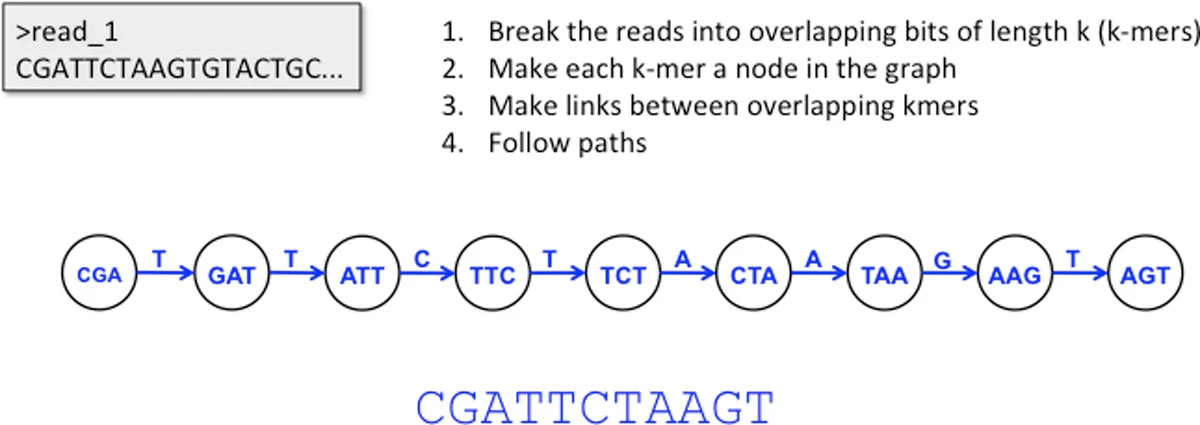
\includegraphics[scale=.3]{images/dBG.png}
  	\caption{Esempio di grafo di \textit{de Bruijn} costruito da k-mer sovrapposti.}
  	\label{fig:dBG}
\end{figure}

\noindent
Poiché i dati sequenziati contengono errori (stimati tra 0.1\% e 1\%) e le ripetizioni genomiche possono essere molto lunghe, gli errori sulle read possono causare vicoli ciechi nel percorso e ripetizioni nel genoma possono causare cicli nel grafo. Una mutazione (SNP) causerà con alta probabilità queste sottostrutture. Perciò concentrandoci su queste strutture, si possono identificare la variazioni direttamente all'interno del grafo. La struttura di base che indica la presenza di un SNP è descritta come una `bolla' (vedi Figura \ref{fig:dBG_bubble}).

\begin{definition}
\label{def:dBG_bubble}
Una bolla è una biforcazione chiusa di un cammino ed è causata da una singola differenza nucleoditica alla fine di un \textit{k}-mer. Partendo da un nodo (sinistro) chiamato \textit{start} è possibile seguire i cammini generati dai due nodi figli $n_h$ e $n_l$ (rispettivamente chiamati \textit{superiore} e \textit{inferiore}) terminando in un nodo (destro) chiamato \textit{end}. Dipendentemente dal tipo di mutazione (SNP) che ha prodotto la bolla, i due cammini possono avere lunghezze diverse. Se il nodo \textit{start} ha più di due nodi figli (destri), tutte le possibili coppie sono trattate come $n_h$ e $n_l$.
\end{definition}

\begin{figure}[h!]
	\centering
  	\captionsetup{justification=centering}
  	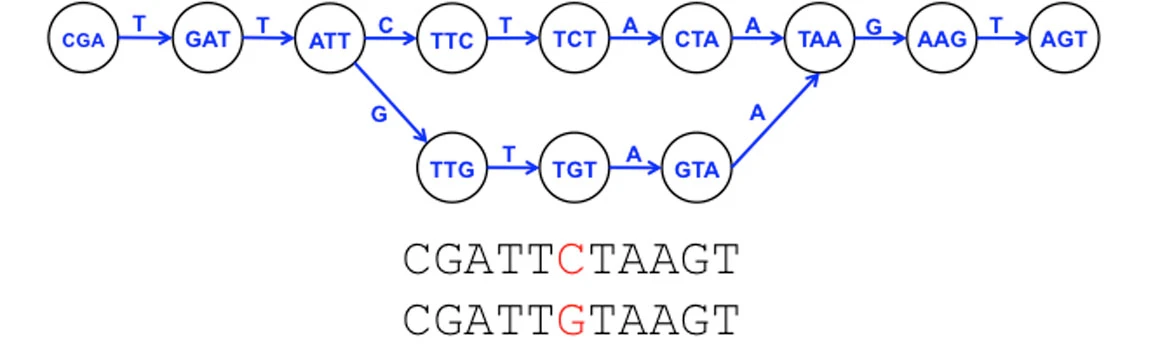
\includegraphics[scale=.3]{images/dBG_bubble.png}
  	\caption{Esempio di bolla all'interno di un grafo di \textit{de Bruijn}.}
  	\label{fig:dBG_bubble}
\end{figure}


\subsubsection{Struttura dati di DiscoSnp\texttt{++}}
\label{dBG_prob}

DiscoSnp\texttt{++} basa la sua efficienza sulla struttura dati Minia \cite{chikhi2013space} che permette di costruire grafi di \textit{de Bruijn probabilistici}. Un grafo di \textit{de Bruijn} probabilistico è ottenuto inserendo tutti i nodi di un grafo di \textit{de Bruijn} all'interno di un Bloom Filter (vedi sezione \ref{BloomFilter}) posti in cascata. All'interno di questa struttura dati, differentemente da un grafo di \textit{Bruijn} classico, gli archi sono dedotti implicitamente dalle interrogazioni fatte ai Bloom Filter per l'appartenenza di tutte le possibili estensioni di un \textit{k}-mer e non necessitano di essere memorizzati. In particolare, un'estensione di un \textit{k}-mer \textit{v} è la concatenazione o (1) di un suffisso di lunghezza $k-1$ di \textit{v} con uno dei quattro possibili nucleotidi o (2) di uno dei quattro nucleotidi con il prefisso di lunghezza $k-1$ di \textit{v}. Un grafo di \textit{de Bruijn} probabilistico possiede un'approssimazione eccessiva del grafo originale e per questo è possibile che, interrogando il Bloom Filter sull'esistenza o meno di un arbitrario nodo del grafo, si ottenga come risposta un elemento falso positivo (ma mai un falso negativo), perciò questa sovra-approssimazione introduce delle diramazioni false tra i nodi originali del grafo e i nodi falsi positivi.

\paragraph{Struttura \textit{cFP}} Per risolvere questo inconveniente,\cite{chikhi2013space} hanno implementato all'interno di Minia un meccanismo per evitare false diramazioni: esso si occupa di individuare e memorizzare gli elementi (\textit{k}-mer falsi positivi) che sono responsabili delle false ramificazioni all'interno di una struttura separata, \textit{cFP} (critical False Positive), implementata tramite la struttura dati che consente rapidi test di appartenenza o meno all'insieme. Ogni interrogazione fatta al Bloom Filter è quindi modificata in modo tale che produca \textit{si} (true) se e solo se il Bloom Filter risponde \textit{si} (true) e se l'elemento su cui si sta interrogando non è presente all'interno di \textit{cFP}. Naturalmente, se \textit{cFp} contenesse tutti i \textit{k}-mer falsi positivi, i vantaggi di usare un Bloom Filter per migliorare l'efficienza dell'uso della memoria andrebbero persi. L'osservazione chiave, risiede nel fatto che i \textit{k}-mer che vengono interrogati mentre si attraversa il grafo non sono tutti i possibili \textit{k}-mer. 

\subparagraph{Osservazione} Sia $S$ l'insieme dei nodi falsi positivi, ed $E$ l'insieme delle estensioni dei nodi da $S$, assumendo che il grafo venga attraversato iniziando da un nodo in $S$, i falsi positivi che non appartengono a $E$ non verranno mai interrogati. Perciò, l'insieme \textit{cFP} sarà un sotto-insieme di $E$. Sia $P$ l'insieme di tutti gli elementi di $E$ per il quale il Bloom Filter risponde \textit{si}. Allora l'insieme \textit{cFP} dei falsi positivi critici è formalmente definito come $cFP = P \setminus S$.

\subsubsection{Algoritmo di DiscoSnp\texttt{++}}
Gli algoritmi presenti all'interno dei moduli di \textsc{DiscoSnp} (\textsc{KisSnp2} e \textsc{KissReads}) sono stati stati rivisitati per ottenere un miglior filtraggio degli errori di sequenziamento in modo da individuare nuove mutazioni (SNP), come analizzeremo in seguito.\\

\noindent
DiscoSnp\texttt{++} è composto da quattro moduli indipendenti (vedi Figura \ref{fig:discosnp_pipe}) che verranno ora enunciati brevemente e poi analizzati in dettaglio. Il primo modulo costruisce il \textit{dBG} dei dataset forniti in input. Successivamente, nel secondo modulo vengono individuate le bolle generate, all'interno del \textit{dBG}, dalle mutazioni e viene prodotto un file FASTA che contiene tutte le variazione presenti in un contig. A seguire, nel terzo modulo vengono mappate le read presenti nei dataset iniziali nel file prodotto dal secondo modulo. Infine, nel quarto modulo viene generato il file VCF delle mutazioni predette che opzionalmente possono essere mappate su un genoma di riferimento, se fornito.

\begin{figure}[h!]
	\centering
  	\captionsetup{justification=centering}
  	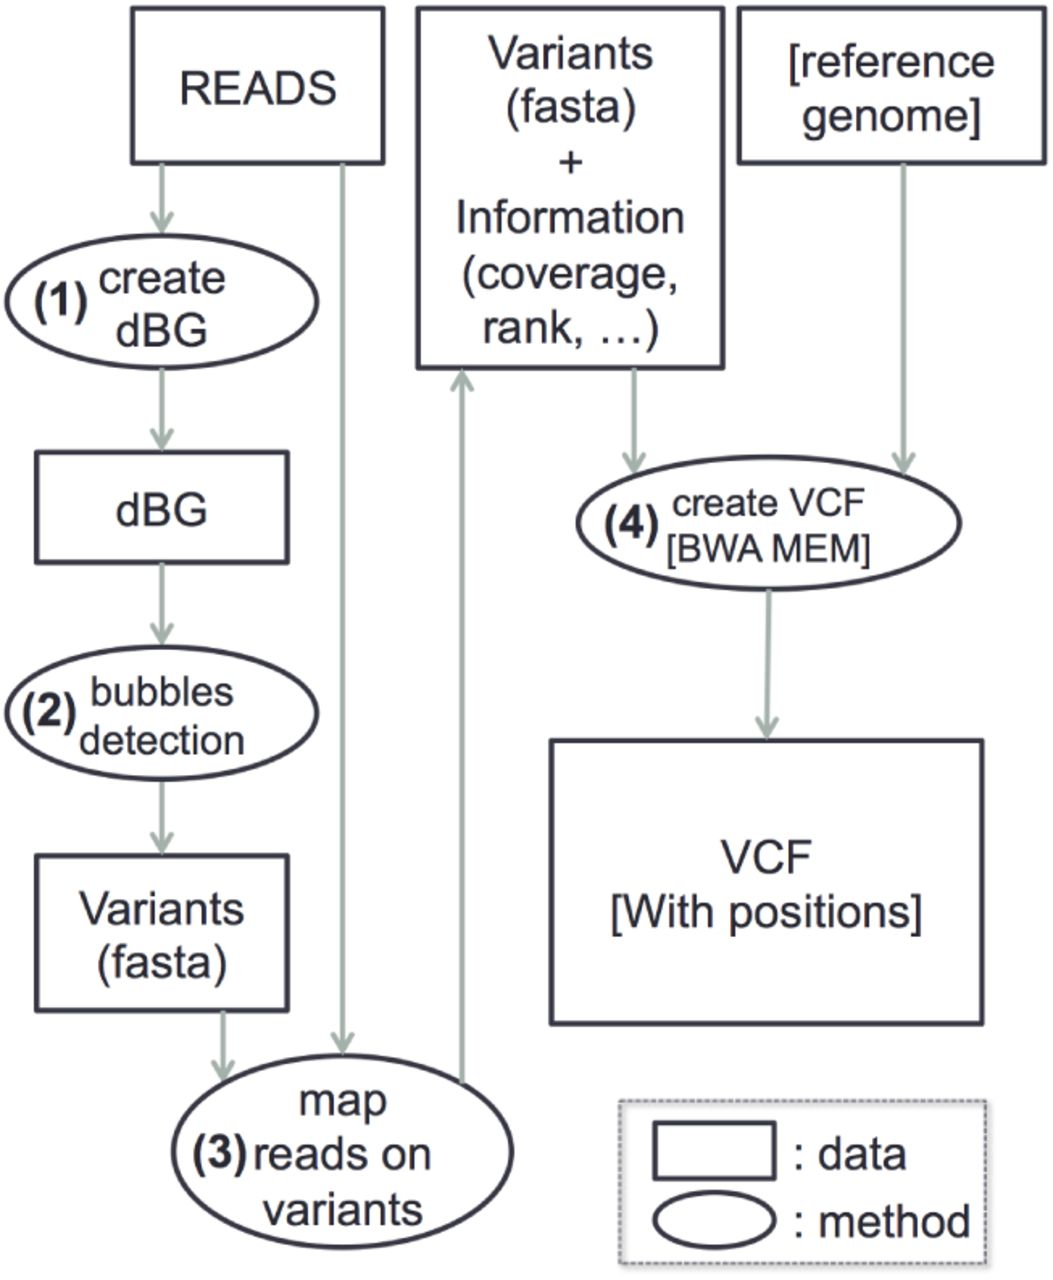
\includegraphics[scale=.7]{images/discosnp_pipeline.jpg}
  	\caption{DiscoSnp\texttt{++} pipeline. Nel caso sia fornito un genoma di riferimento, il VCF file conterrà anche il posizionamento delle previsioni mappate.}
  	\label{fig:discosnp_pipe}
\end{figure}

\paragraph{Modulo 1} Una volta ricevuti in ingresso i dataset, grazie alla struttura dati discussa nella Sezione \ref{dBG_prob} e la libreria GATB (Genome Analysis Toolbox with \textit{de-Bruijn} graph) si costruisce il grafo. Nello specifico, a causa degli errori di sequenziamento prodotti dagli NGS, ogni \textit{k}-mer può avere al più \textit{k} errori ed uno step cruciale nella costruzione del grafo risulta essere la rimozione di questi \textit{k}-mer. La rimozione è fatta tramite un classico approccio di conteggio di \textit{k}-mer usando l'algoritmo KMC2, implementato usando la libreria GATB. Perciò, tutti i \textit{k}-mer che hanno un numero di occorrenze non superiore ad una threshold $T_{sol}$\footnote{\ DiscoSnp\texttt{++} definisce una threshold di solidità indipendente per ogni insieme di read. Più precisamente, per ogni insieme di read, il parametro $T_{sol}$ (ottimo) è dedotto automaticamente dall'istogramma che rappresenta la quantità di ogni \textit{k}-mer (``\textit{k}-mer abundances''). Per fare ciò, la seguente euristica viene applicata: si leviga l'istogramma, si cerca la posizione in cui si presentano il primo incremento e il massimo valore raggiunto successivamente, si cerca infine l'indice del valore minimo tra queste due posizioni. L'indice così trovato è il valore di soglia dedotto automaticamente e corrisponde approssimativamente alla distanza tra un \textit{k}-mer errato e un \textit{k}-mer solido. Questa euristica assicura che non più del 25\% dei \textit{k}-mer distinti sono sotto questo valore di soglia, e che normalmente questo valore è $\geq3$.}, detta di solidità, vengono rimossi. Se  un \textit{k}-mer possiede un numero di occorrenze maggiore di ogni altro valore di threshold degli insiemi di read è considerato solido e viene memorizzato all'interno del grafo, altrimenti viene scartato.

\paragraph{Modulo 2} Il secondo modulo, si occupa di individuare e classificare le bolle (vedi Definizione \ref{def:dBG_bubble}) generate dalla presenza di SNP (vicini o meno) e/o indel all'interno del grafo, ovvero ricercare la presenza di due path distinti formati da $k+2$ nodi, che hanno in comune i \textit{nodi di diramazione}\footnote{\ Un nodo di diramazione, o \textit{branching node}, è un nodo che ha più di un predecessore e/o più di un successore.} iniziale e finale, tramite due algoritmi. Prima di procedere con la spiegazione degli algoritmi è utile definire alcuni concetti.

\begin{definition}
Una bolla si definisce \textit{ramificata} quando almeno uno dei due path generati da $n_h$ e $n_l$ contiene un \textit{branching node}. Sono esclusi da questa caratterizzazione i nodi \textit{start} ed \textit{end} della bolla.
\end{definition}

\begin{definition}
Una bolla ramificata si definisce \textit{simmetrica} se più di due cammini possono essere percorsi simultaneamente partendo dai nodi $n_h$ e $n_l$. Al contrario una bolla ramificata si definisce \textit{non simmetrica} se dai nodi $n_h$ e $n_l$ esistono esattamente due cammini (superiore e inferiore) che convergono ad un \textit{branching node} di destinazione.
\end{definition}

\paragraph{Osservazione} Se i cammini $n_h$ e $n_l$ sono composti da esattamente $k$ nodi, allora si tratta di una mutazione \textit{isolata} in quanto non esistono altri polimorfismi, e quindi \textit{branching node}, nei $k$ nucleotidi prima e dopo la posizione della mutazione. Se invece la bolla generata presenta due cammini con lo stesso numero di nodi, maggiore di $k$, siamo in presenza di una variazione \textit{non isolata}. Nel caso i cammini generati da $n_h$ e $n_l$ si presentano con un diverso numero di nodi, siamo in presenza di indel. Solitamente il cammino di lunghezza minima prodotto ha esattamente $k-1$ nodi, ma dipendentemente dal contesto in cui si verifica la lunghezza può variare ed essere inferiore a $k-1$\footnote{\ Accade quando l'indel e ciò che lo segue (o precede) hanno un prefisso (o suffisso) comune di dimensione $> 0$. Più precisamente, se le dimensioni di prefisso e suffisso sono rispettivamente $p_1$ e $p_2$, il cammino di lunghezza minima è composto da $max(0, k-1-p_1 - p_2)$ nodi e quello di lunghezza massima è composto da ($k-1+d-p_1 - p_2$) con $d$ dimensione dell'indel.}.\\

\noindent
Siamo ora pronti ad analizzare gli algoritmi che vengono implementati all'interno di questo secondo modulo. Il primo algoritmo, attraversando tutti i \textit{k}-mer che presentano un nodo di diramazione destro, li propone inizialmente come potenziali nodi di partenza per bolle che identificano SNP e nel caso non lo siano li propone come potenziali nodi di partenza per bolle che identificano indel. In questo secondo caso, tutte le possibili combinazioni di indel vengono proposte, dato che l'inserimento può avvenire nel cammino inferiore o superiore e può avere una dimensione variabile (non può superare la dimensione massima autorizzata dall'utente). Per ogni \textit{k}-mer (SNP o indel) proposto dall'algoritmo precedente, il secondo algoritmo (ricorsivo) espande congiuntamente due cammini e controlla che i vincoli imposti sui parametri\footnote{\ Tramite i parametri di \textit{branching}, è possibile limitare la ricerca alle sole bolle non ramificate, o alle bolle non ramificate o non simmetriche, o a qualunque tipo di bolla senza restizioni.} di diramazione siano rispettati. Se i due \textit{k}-mer che si stanno espandendo sono identici, allora la bolla è giunta alla fine, altrimenti la ricorsione continua. Qualunque sia il risultato dell'espansione, l'algoritmo controlla l'esistenza di potenziali \textit{k}-mer di chiusura $k\texttt{-}mer_1$ e $k\texttt{-}mer_2$ che possono essere estesi con caratteri differenti $\alpha$ e $\beta$. Processati tutti i nodi proposti, viene generato un file FASTA contenente le mutazioni trovate.

\paragraph{Modulo 3} Per mantenere basso l'utilizzo della RAM, nessun'altra informazione oltre al \textit{k}-mer viene memorizzata nel \textit{dBG}; per questo motivo le varianti trovate dal modulo precedente non hanno nessuna informazione in merito alla frequenza di ogni \textit{k}-mer nei dataset iniziali. Perciò, questo modulo si occupa di mappare le read iniziali sulle sequenze delle mutazioni trovate, in modo da determinare la copertura delle read per allele e per ogni variante dentro i dataset. Oltre a queste statistiche, dipendentemente dal numero di dataset (tipicamente $\geq2$) confrontati, viene calcolato il rank di ogni mutazione\footnote{\ Il rank di ogni mutazione viene valutato tramite il coefficiente Phi, il quale misura l'associazione tra due variabili binarie. È anche chiamato \textit{Mean Square Contingency Coefficient}, usato insieme alle tabelle di contingenza (chiamate anche tabelle a campi incrociati o tabelle a due vie) per riepilogare la relazione tra diverse variabili osservate.} nel seguente modo: $max\left( \binom{m}{2}\sqrt{\frac{\chi^2}{n}}\ \right)$, con \textit{n} somma della frequenza della read, \textit{m} numero dei dataset e $\chi$ coefficiente Phi della tabella di contingenza dei conteggi delle read. I genotipi vengono dedotti in modo indipendente per ogni organismo, tramite la copertura delle read per allele. Per fare ciò, le probabilità dei tre possibili genotipi (due omozigoti o eterozigote) vengono calcolate tramite un semplice modello binomiale, basato sul parametro \textit{err}, che rappresenta la probabilità che una read venga mappata erroneamente su un allele; si assume che questa probabilità sia fissata ($0.01$) e indipendente in ogni osservazione. Il genotipo che presenta la probabilità più alta viene scelto e fornito in output insieme a tutte le altre probabilità calcolate. Finito il processo viene generato un file contenente le informazioni legate al file FASTA prodotto dal secondo modulo.

%\begin{equation}
%like_{0/0} = -10\log_{10}{\left( (1-err)^{c_u} \times err^{c_l} \times C^{c_u}_{c_u + c_l} \times \frac{1-prior}{2} \right)}
%\end{equation}
%
%\begin{equation}
%like_{1/1} = -10\log_{10}{\left( err^{c_u} \times (1-err)^{c_l} \times C^{c_u}_{c_u + c_l} \times \frac{1-prior}{2} \right)}
%\end{equation}
%
%\begin{equation}
%like_{0/1} = -10\log_{10}{\left( \left(\frac{1}{2}\right)^{c_u + c_l} \times prior \right)}
%\end{equation}
%
%\begin{equation}
%min\left( like_{0/0},like_{1/1},like_{0/1} \right) \Rightarrow 0/0\ ,1/1\ ,0/1
%\end{equation}

\paragraph{Modulo 4} Quest'ultimo modulo genera il file VCF delle varianti predette. Se nessun genoma di riferimento è fornito, questo modulo si limita a cambiare il formato dei file prodotti dai moduli 2 e 3 da FASTA a VCF. Altrimenti, utilizzando l'algoritmo BWA-mem (che esegue l'allineamento locale) le mutazioni predette vengono mappate sul genoma di riferimento e questo permette di localizzare ogni variante nel genoma. Se una variante ha più di una posizione ottima di mappatura, ne viene scelta una random (ma viene comunque segnalata la presenza di possibili mappature multiple in un campo del file VCF).

\end{document}
